The \texttt{\pkglnk{model}} package contains the \texttt{\lnk{ExecutionEngine}}
class, which is the primary interface provided by the model to the view for working
with lambda terms. It is initialized with an input string, as well as the reduction
order (see \texttt{\pkglnk{model.reduction}}), output size (see \texttt{\pkglnk{model.output}})
and libraries (see \texttt{\pkglnk{model.library}}) to be used and can then be used to
interactively operate on the lambda term, by stepping forward (that is, $\beta$-reducing
according to the reduction order or reducing a provided redex in the current term)
and backward (reverting to the previous term that was displayed).

The \texttt{\lnk{ExecutionEngine}} is fully synchronous and does not have a notion
of "fully" reducing a term.

\begin{figure}[H]
	\centering
	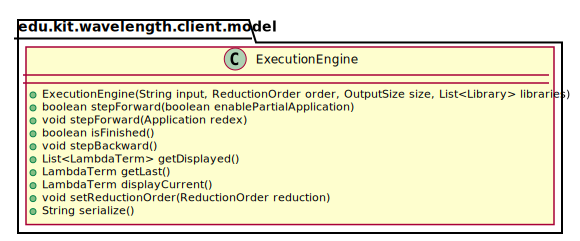
\includegraphics[width=\textwidth]{packageDiagrams/modelPackage}
\end{figure}
